\documentclass[12pt]{report}
\usepackage{multirow}
\usepackage{doublespace}
\usepackage{csmthesis}
\usepackage{aaai-bib}
\usepackage{caption}
\usepackage{algorithm}
\usepackage[noend]{algpseudocode}
%Place content-specific packages
\usepackage{mathtools}
\usepackage{amsmath}
\usepackage{times}
\usepackage{helvet}
\usepackage{courier}
\usepackage{pbox}
\usepackage{caption}
\usepackage{subcaption}
\captionsetup{compatibility=false}
\usepackage{amssymb}% http://ctan.org/pkg/amssymb
\usepackage{pifont}% http://ctan.org/pkg/pifont
\usepackage{array,booktabs}
\newcolumntype{L}{@{}>{\kern\tabcolsep}l<{\kern\tabcolsep}}
\usepackage{colortbl}
\usepackage{xcolor}
\usepackage{tikz}
\usetikzlibrary{matrix}
%\usepackage{epsfig}
\usepackage{graphicx}
%\usepackage{subfigure}
\graphicspath{ {./images} }
%\usepackage{xspace}
%\usepackage[leqno]{amsmath}
%\usepackage{amssymb}
%\usepackage{dsfont}

%\bibliographystyle{mlapa}

\usepackage{geometry}
\geometry{verbose, letterpaper, dvips, tmargin=1in, lmargin=1.6in, rmargin=0.9in, bmargin=1in, total={6in,9in}, includeheadfoot, headsep=12pt}



\tikzset{ 
    table/.style={
        matrix of nodes,
        row sep=-\pgflinewidth,
        column sep=-\pgflinewidth,
        nodes={
            rectangle,
            draw=black,
            align=center
        },
        minimum height=1.5em,
        text depth=0.5ex,
        text height=2ex,
        nodes in empty cells,
%%
        every even row/.style={
            nodes={fill=gray!20}
        },
        column 1/.style={
            nodes={text width=3em,font=\bfseries}
        },
        row 1/.style={
            nodes={
                fill=black,
                text=white,
                font=\bfseries
            }
        }
    }
}

\newcommand{\etal}{et al.\xspace}
\newcommand{\eg}{e.g.,\xspace}
\newcommand{\comment}[1]{}
\newcommand{\cmark}{\ding{51}}%
\newcommand{\xmark}{\ding{55}}%
\def\newnot#1{\label{#1}}

\def\ni{\noindent}
\newcommand{\header}[1]{\noindent \bf{#1}\rm \\ \ni }
\input{psfig.tex}

\begin{document}
\title{{\bf THESIS-TITLE}}
\author{MY-FULL-NAME}
\tolerance=1000
\newpage
\newpage
\begin{titlepage}
\vspace{0.6in}
\begin{singlespace}

\begin{center}
\vspace{0.1in}
\large{\bf APPROVAL SHEET}
\bigskip \bigskip
\end{center}

\begin{flushleft}
{\bf Title of Thesis:}{\hspace{3mm}}Recoloring Web Pages For Color Vision Deficiency Users.\\
\vspace{0.5in}
{\bf Name of Candidate:}{\hspace{3mm}} \parbox[t]{2in}{Vikas Bansal \\ Masters in Science, 2014}
\end{flushleft}

\vspace{0.5in}

\begin{flushleft}
{\bf Thesis and Abstract Approved:}{\hspace{3mm}} 
\parbox[t]{2.5in}{\underline{\hspace{2.0in}}\\ 
	Dr. Tim Finin\\
	Professor \\
	Department of Computer Science and \\
	Electrical Engineering}
\end{flushleft}
\vspace{0.5in}
\begin{flushleft}
{\hspace{59.9mm}}\parbox[t]{2.5in}{\underline{\hspace{2.0in}}\\ 
	Dr. Lina Zhou\\
	Associate Professor \\
	Department of Information Systems}
\end{flushleft}

\vspace{0.8in}

\begin{flushleft}
{\bf Date Approved:}{\hspace{3mm}} \underline{\hspace{2.5in}}\\
\end{flushleft}

\end{singlespace}
\end{titlepage}
\par\vfil

\newpage
\begin{titlepage}

\begin{center}
\vspace{0.1in}
\large{\bf Curriculum Vitae}
\bigskip \bigskip
\end{center}

\begin{flushleft}
  {\bf Name:}{\hspace{3mm}}Vikas Bansal.\\
	{\bf Permanent Address:}{\hspace{3mm}} 130 Forest St, Stamford, CT 06901. \\
	{\bf Degree and date to be conferred:}{\hspace{3mm}}Masters in Science, May 2014. \\
	{\bf Date of Birth:}{\hspace{3mm}}01/27/1991. \\
	{\bf Place of Birth:}{\hspace{3mm}}India. \\
	{\bf Secondary Education:}{\hspace{3mm}} Columbia Foundation Senior Secondary School, New Delhi, New Delhi.\\
	{\bf Collegiate institutions attended:}\\
	\begin{singlespace} 
	{\hspace{0.4in}}University of Maryland Baltimore County, Masters in Science Computer Science, 2014. \\
	{\hspace{0.4in}}\parbox[t]{5.5in}{LNMIIT, Bachelor of Technology (Hons.) Electronics and Communication Engineering, 2012} \\
	\end{singlespace} 
	\vspace{8pt}
	{\bf Major:}{\hspace{3mm}}Computer Science.\\
	{\bf Minor:}{\hspace{3mm}}Computer Science.\\
	% {\bf Professional publications:}\\
	% \begin{singlespace} 
 %  {\hspace{0.4in}} \parbox[t]{5.5in}{FULL-CITATION-INFORMATION.}\\
 %  {\vspace{5pt}}
 %  {\hspace{0.4in}} \parbox[t]{5.5in}{FULL-CITATION-INFORMATION.}\\
 %  \end{singlespace} 
 %  \vspace{8pt}
	{\bf Professional positions held:}\\
	\begin{singlespace}
	{\hspace{0.4in}}\parbox[t]{5.5in}{Intern at Xerox Corporation. (May 28, 2013 -- August 23, 2013).}\\
	{\vspace{5pt}}
	{\hspace{0.4in}}\parbox[t]{5.5in}{Research Assistant at UMBC. (January 13, 2013 -- June 30, 2014).}\\
	{\vspace{5pt}}
	{\hspace{0.4in}}\parbox[t]{5.5in}{Teaching Assistant at UMBC. (January 20, 2014 -- May 21, 2014).}\\
	\end{singlespace}
\end{flushleft}
       
\end{titlepage}
\par\vfil



\newpage
\newpage
\pagestyle{empty}

\begin{center}
\vspace{0.1in}
\large{\bf ABSTRACT} \par  
\bigskip \bigskip
\end{center}

\begin{flushleft}
{\bf Title of Thesis:} Recoloring Web Pages For Color Vision Deficiency Users.\\
Vikas Bansal, Masters in Science, 2014 \\
\begin{singlespace}
{\bf Thesis directed by:}{\hspace{2.5mm}} \parbox[t]{3in}{Dr. Lina Zhou, Associate Professor\\
Department of Information Systems}
\end{singlespace}
\begin{singlespace}
{\hspace{37.9mm}}\parbox[t]{3in}{Dr. Tim Finin, Professor\\
Department of Computer Science and \\ Electrical Engineering}
\end{singlespace}
\end{flushleft}

Colors are an important part of our life. They are commonly used to represent important information, specially, categories. Ability to differentiate between colors is important in performing routine tasks such as reading content, following traffic lights etc. This ability varies from person to person. Many people experience difficulty in reading content on web pages due to this variation. These difficulties result from the inability of individuals to sufficiently differentiate between colors. This condition of an individual is called Color Vision Deficiency (CVD). More than four percent of current population suffer from some kind of CVD, significantly affecting their web experience.

To improve the web experience of CVD users, we have presented an algorithm which can be used to recolor web pages such that the recolored web pages do not pose any difficulty to a CVD user. Replaced colors are chosen from a fixed set of color called Dichromacy Trichromacy Equivalency Plane (DTEP) set. While recoloring we also preserve the naturalness and contrast among foreground and background colors in different sections of the web page. A quantitative comparison with the existing tool SPRWeb[] shows that our algorithm performs better in preserving contrast among different sections of the web pages and doesn’t differ much in preserving naturalness.

An additional step in to algorithm was added to induce the contrast in pairs according to the W3C guidelines. Quantitative experimentation of modified algorithm shows that contrast ratio in each replacement pair is more than 4.5 as required for readability. 

\par\vfil


\newpage
\begin{titlepage}
\mbox{}\vspace{1in}
\begin{center}

    {\Large \bf Recoloring Web Pages For Color Vision Deficiency Users. \par}
    
\vspace{2in}

    {\large by} \\
    {\large Vikas Bansal}
    
\vspace{2in}

  \begin{singlespace}
    Thesis submitted to the Faculty of the Graduate School \\
    of the University of Maryland in partial fulfillment \\
    of the requirements for the degree of \\
    Masters in Science \\
    2014
	\end{singlespace}
\end{center}
\end{titlepage}

\newpage
\begin{titlepage}
\mbox{}\vspace{7.5in}
\begin{center}
\copyright~Copyright Vikas Bansal 2014
\end{center}
\end{titlepage}


%\frontmatter
\pagenumbering{roman}

\newpage
\setcounter{page}{2}
\cleardoublepage
\newpage
\newpage
\fchapter[Dedication]{}
\thispagestyle{plain}
%\begin{titlepage}
\vfil\null
\begin{center}

\mbox{}\vspace{3in}

\emph{I dedicate this thesis to mom, dad, Rajesh chacha and me.}

\end{center} 
\normalsize
\vfil\null
%\end{titlepage}

\cleardoublepage
\fchapter{ACKNOWLEDGMENTS}
\pagestyle{plain}

I am very thankful to Dr. Lina Zhou, Dr. Dongsong Zhang and Dr. Tim Finin for their time and contribution. They are really good professors and were helpful to me through my entire research time. Not only did they teach me how to be a good researcher, but also they showed me how to use time effectively and efficiently to get the expected goal. 

Besides, I am very grateful to my friends, specially, Primal Pappachan, Manik Budhiraja and Akshay Grover for their support. 

Finally, I would like to thank my family for all kinds of supports. Life would have been very difficult without them.  
\cleardoublepage
\tableofcontents
\cleardoublepage
\listoffigures
\cleardoublepage
\listoftables
\cleardoublepage

%\mainmatter
\pagenumbering{arabic}
\pagestyle{myheadings}
\markright{}

\chapter{Introduction}
\thispagestyle{plain}

\label{Introduction}
Website colors specially which are used in foreground text and background are responsible to provide legibility in the content. In addition to providing legibility, they also influence the subjective responses from the users. Depending on the color, a website may seem heavy or light, high or low in temperature and may tell about busyness.

While one solution to the problem of illegibility could be to educate web designers so that they only use a set of colors which are comfortable to both CVD and normal users. [we have developed one such technique - webpages colors downloaded]. Which is a kind of a prevention step. One such color combination could be to develop all the webpages using only black and white. But that itself defeats the purpose of existence of colors. Most of the web developers today, even being aware of the existence of CVD users, develop web pages considering only normal web users leading to confusion and frustration among CVD users.

Another solution is more of a rectifying step. In this, we recolor existing ‘bad web pages’ to suit the need of both normal and CVD users.
\section{SECTION-TITLE}
\label{SECTION-LABEL}

\section{SECTION-TITLE}
\label{SECTION-LABEL}

\subsection{SECTION-TITLE}
\label{SECTION-LABEL}

\subsection{SECTION-TITLE}
\label{SECTION-LABEL}
\cleardoublepage
\chapter{Background and Related Work}
\thispagestyle{plain}

\label{Background and Related Work}

In this section we will learn about CVD and the existing related work to deal with it. Which also formed the basis of this thesis.

\section{Color Vision Deficiency (C.V.D.)}
\label{Color Vision Deficiency}


Color vision deficiency [1], is the inability or decreased ability to see color, or perceive color differences, under normal lighting conditions. Color blindness affects a significant percentage of the population [2].  There is no actual blindness but there is a deficiency of color vision. The most usual cause is a fault in the development of one or more sets of retinal cones that perceive color in light and transmit that information to the optic nerve. This type of color blindness is usually a sex-linked condition. The genes that produce photo-pigments are carried on the X chromosome; if some of these genes are missing or damaged, color blindness will be expressed in males with a higher probability than in females because males only have one X chromosome (in females, a functional gene on only one of the two X chromosomes is sufficient to yield the needed photo-pigments).

Color blindness can also be produced by physical or chemical damage to the eye, the optic nerve, or parts of the brain. For example, people with achromatopsia suffer from a completely different disorder, but are nevertheless unable to see colors.

By cause CVD can be classified in to three types:
\begin{itemize}
\item{Acquired}
\item{Inherited:} Inherited can further be classified in to three types:
\begin{itemize}
\item{Monochromacy:} Also known as "total color blindness", is the lack of ability to distinguish colors (and thus the person views everything as if it were on a black and white television); caused by cone defect or absence. Monochromacy occurs when two or all three of the cone pigments are missing and color and lightness vision is reduced to one dimension. We are not dealing with this type in our current version of the algorithm.
\item{Dichromacy:} Dichromacy is a moderately severe color vision defect in which one of the three basic color mechanisms is absent or not functioning. Our algorithm can recolor web pages to suit all the Dichromats.
\begin{itemize}
\item{Protanopia (1\% of the males):} Protanopia is a severe type of color vision deficiency caused by the complete absence of red retinal photoreceptors. It is a form of dichromatism in which the subject can only perceive light wavelengths from 400 to 650nm, instead of the usual 700nm. Pure reds cannot be seen, instead appearing black; purple colors cannot be distinguished from blues; more orange-tinted reds may appear as very dim yellows, and all orange-yellow-green shades of too long a wavelength to stimulate the blue receptors appear as a similar yellow hue. It is hereditary and sex-linked.
\item{Deuteranopia (1\% of the males):} Deuteranopia is a color vision deficiency in which the green retinal photoreceptors are absent, moderately affecting red–green hue discrimination. It is a form of dichromatism in which there are only two cone pigments present. It is likewise hereditary and sex-linked.
\item{Tritanopia (Less than 1\% of males and females):} Tritanopia is a very rare color vision disturbance in which there are only two cone pigments present and a total absence of blue retinal receptors. Blues appear greenish, yellows and oranges appear pinkish, and purple colors appear deep red. It is related to Chromosome "7".
\end{itemize}
\item{Anomalous trichromacy}
\end{itemize}
\end{itemize}

\section{Diagnosis}
\label{Diagnosis}

The Ishihara color test [14], which consists of a series of pictures of colored spots, is the test most often used to diagnose red–green color deficiencies. A figure (usually one or more Arabic digits) is embedded in the picture as a number of spots in a slightly different color, and can be seen with normal color vision, but not with a particular color defect. The full set of tests has a variety of figure/background color combinations, and enable diagnosis of which particular visual defect is present.

To test the type of color blindness users have, we did the Ishihara color test on each of them during our user study of the algorithm.

% \begin{figure}[p]
% 	\includegraphics{Ishihara1.PNG}	    
% \end{figure}

\begin{figure}
\centering
\begin{subfigure}{.5\textwidth}
  \centering
  \includegraphics[width=.5\linewidth]{Ishihara1.PNG}
  \caption{Plate No. 1 (12)}
  \label{fig:sub1}
\end{subfigure}%
\begin{subfigure}{.5\textwidth}
  \centering
  \includegraphics[width=.5\linewidth]{Ishihara2.PNG}
  \caption{Plate No. 13 (6)}
  \label{fig:sub2}
\end{subfigure}
\caption{Ishihara Test}
\label{fig:test}
\end{figure}

% {\vspace{10mm}}
% \includegraphics[width=0.4\linewidth]{Ishihara1.PNG}
% \captionof{figure}{Ishihara Plate No. 1 (12) [Wikipaedia]}


\section{Related Work}
\label{Related Work}

Quite a work has been done to both simulate and correct CVD. Ichikawa et al. [7] were the first publishers of a website recolouring tool that improves accessibility for people with CVD. Iaccarino et al. [21] proposed the use of edge services to recolour website images in transit to the user. ColorBlindnessSimulateCorrect by Seewald Solutions [8] is one of the examples of an application developed to both simulate and correct CVD effect. It uses a linear transformation on rgb input. ‘Daltonize’ developed by www.daltonize.org [9] can be used to recolor web pages. They first convert RGB values of a color to LMS values and then compensate for color blindness by shifting wavelengths away from the portion of the spectrum invisible to the dichromat, towards the visible portion.  Eyepilot [20] enables computer users with red-green color blindness to decipher color-coded maps and graphs by letting the user place a floating window on top of any picture to distinguish among the various color fields. The GNOME [19] desktop environment provides users with the option to switch a color filter on and off choosing from a set of possible color transformations that displace the colors in order to disambiguate them. While all these tools have proved to be effective in inducing differentiability in the content and thus providing legibility, but none of them have been able to retain the naturalness, differentiability of the original web page.

One such tool which preserves naturalness and improves color differentiability is kuhn’s [10 ]tool. One improvement on naturalness preservation was done by David et al. in SPRWeb [6]. Which is also the basis of this thesis. SPRWeb performs better in preserving naturalness and differentiability than Kuhn’s tool. But it fails to make sure than all the foreground background color pairs have the minimum required contrast ratio threshold of 4.5 as per W3C guidelines.

\section{Definitions}
\label{Related Work}
\begin{itemize}
\item{\textbf{O}: } Original set of colors as parsed from CSS files associated with the web page.
\item{\textbf{R}: } Replaced set of colors as computed by the recoloring algorithm. And obviously, size of \textbf{R} is always equal to size of \textbf{O}.
\item{\textbf{P}: } Number of color \textit{pairs} in a web page. A \textit{pair} of colors from a web page is of the form \textit{(fg,bg)}, where \textit{fg} is a foreground text color and \textit{bg} is a background color. There can be many such \textit{(fg,bg)} color pairs. 
\item{\textbf{Perceptual naturalness[6]: }} It is a measure of how close is set \textbf{R} to set \textbf{O}. Ideally, if our algorithm is able to find a set such that \textbf{R} = \textbf{O} then the \textit{perceptual naturalness} will be maximum and the \textit{cost of naturalness} would be 0. \textit{Cost of naturalness} quantifies naturalness factor. As defined in SPRWeb, \textit{cost of naturalness} can be quantified using the following expression:

\begin{figure}[!htb]
  \centering
\[ pn = \frac{1}{N}*\sum_{i=1}^{N} \Delta_{L_{ab}}(O_{i},R_{i})\]
  \begin{tabular}{@{}>{$}l<{$}l@{}}
    N & Size of \textbf{O}.\\
    \Delta_{L_{ab}} & Euclidean distance in Lab color space. \\
  \end{tabular}
\end{figure}



Lab color space [15][16] is explained in the next section. A \textit{low} value of \textit{pn} is highly desirable. A \textit{low} value of \textit{pn} as compared to a high value, essentially tells us that the recolored web page having \textit{low} value is closer to original web page in terms of colors. 
Optimizing the value of \textit{pn} while computing the recolored set \textbf{R} makes sure that the recolored version does not have abrupt colors as compared to the original version. 

\item{\textbf{Perceptual differentiability[6]: }} This factor maintains the differentiability among colors belonging to a pair in the original web page. Suppose the original web page has only one color pair, i.e size of \textbf{P} is 1. And the pair is \textit{(Red,White)}, then the recolored pair should have colors such that the difference in original pair should be maintained to its best possible extent. This factor can be quantified using the following equation:



\begin{figure}[!htb]
  \centering
\[ pd = \frac{1}{size(\textbf{P})}*\sum_{ (X,Y)\in P_{O},P_{R}}^{} |\Delta_{L_{ab}}(X_{f},X_{g}) - \Delta_{L_{ab}}(Y_{f},Y_{g}) |\]
  \begin{tabular}{@{}>{$}l<{$}l@{}}
    P_{O} & Set of pairs in original web page.\\
    P_{R} & Set of pairs in recolored web page. \\
    X & A pair of color in original web page thus a member of $P_{O}$.\\
    Y & Replacement of color pair X thus a member of $P_{R}$.\\
    X_{f} and Y_{f} & \textit{fg} in pair X and Y respectively.\\
  	X_{g} and Y_{g} & \textit{bg} in pair X and Y respectively. \\
  \end{tabular}
\end{figure}

\item{\textbf{Subjective naturalness[6]: }} We need this factor in optimizing function to keep the subjective responses of users as is. For example, using this in optimization we can keep \textit{warm} colors \textit{warm} or \textit{heavy} colors \textit{heavy}. We are using subjective response model developed by Ou [11] to compute the subjectivity factor. To preserve subjectivity of colors in original web page, we use \textit{subjective response space}. We discuss \textit{subjective response space} in detail in future sections. Subjective naturalness cost can be quantified as follows:

\begin{figure}[!htb]
  \centering
\[ srn = \frac{1}{N}*\sum_{i=1}^{N} \O_{u}(O_{i},R_{i})\]
  \begin{tabular}{@{}>{$}l<{$}l@{}}
    N & Size of \textbf{O}.\\
    \O_{u} & Euclidean distance in subjective response space. \\
  \end{tabular}
\end{figure}

\item{\textbf{Subjective differentiability[6]: }} Similar to perceptual differentiability, subjective differentiability should be maintained among pairs of colors parsed from original web page. We again use \textit{subjective response space} to quantify this factor as follows:

\begin{figure}[!htb]
  \centering
\[ spd = \frac{1}{size(\textbf{P})}*\sum_{ (X,Y)\in P_{O},P_{R}}^{} |\O_{u}(X_{f},X_{g}) - \O_{u}(Y_{f},Y_{g}) |\]
  \begin{tabular}{@{}>{$}l<{$}l@{}}
    P_{O} & Set of pairs in original web page.\\
    P_{R} & Set of pairs in recolored web page. \\
    X & A pair of color in original web page thus a member of $P_{O}$.\\
    Y & Replacement of color pair X thus a member of $P_{R}$.\\
    X_{f} and Y_{f} & \textit{fg} in pair X and Y respectively.\\
  	X_{g} and Y_{g} & \textit{bg} in pair X and Y respectively. \\
  \end{tabular}
\end{figure}

\item{\textbf{Cost function: }} = $W_{pn}*pn$ + $W_{pd}*pd$ + $W_{spn}*spn$ + $W_{spd}*spd$

Where $W_{ii}'s$ are weights corresponding to the factors. We can choose any value for these factors depending upon the requirement. We keep a value 1 for all of them to treat all factors equally.    

\section{Color spaces}
\label{color spaces}

\item{\textbf{Lab color space [15][16]: }} A Lab color space is a color-opponent space with dimension L for lightness and a and b for the color-opponent dimensions, based on nonlinearly compressed CIE XYZ color space coordinates. The three coordinates of CIELAB represent the lightness of the color (L\textsuperscript{*} = 0 yields black and L\textsuperscript{*} = 100 indicates diffuse white; specular white may be higher), its position between red/magenta and green (a\textsuperscript{*}, negative values indicate green while positive values indicate magenta) and its position between yellow and blue (b\textsuperscript{*}, negative values indicate blue and positive values indicate yellow). The range of the three coordinates is as follows:
\begin{figure}[!htb]
  \centering
\begin{tabular}{@{}>{$}l<{$}l@{}}
    L\textsuperscript{*}\in&[0,100]\\
    a\textsuperscript{*}\in&[-127,128] \\
    b\textsuperscript{*}\in&[-127,128]\\
  \end{tabular}
\end{figure}

\textbf{Why did we use Lab color space? }\\
\begin{itemize} 
\item{Lab color is designed to approximate human vision. It aspires to perceptual uniformity, and its L\textsuperscript{*} component closely matches human perception of lightness.}
\item{The L\textsuperscript{*}a\textsuperscript{*}b\textsuperscript{*} color space includes all perceivable colors which means that its gamut exceeds those of the RGB and CMYK color models (for example, ProPhoto RGB includes about 90\% all perceivable colors).}
\item{One of the most important attributes of the L\textsuperscript{*}a\textsuperscript{*}b\textsuperscript{*}-model is device independence. This means that the colors are defined independent of their nature of creation or the device they are displayed on. The L\textsuperscript{*}a\textsuperscript{*}b\textsuperscript{*} color space is used e.g. in Adobe Photoshop when graphics for print have to be converted from RGB to CMYK, as the L\textsuperscript{*}a\textsuperscript{*}b\textsuperscript{*} gamut includes both the RGB and CMYK gamut.}
\end{itemize}

\item{\textbf{Subjective response space [11] : }} \textit{Subjective response space} consists of three dimensions which can be formulated as follows using Ou's model [11]:


\begin{figure}[!htb]
Activity(Active, Passive):
\[ AP = -2.1+0.06\sqrt{(L\textsuperscript{*}-50)^{2} + (a\textsuperscript{*}-3)^{2} + (\frac{b\textsuperscript{*}-17}{1.4})^{2}} \]
\end{figure}


\begin{figure}[!htb]
Temperature(Warm, Cool):
\[ WC = -0.5+0.02(C\textsuperscript{*})^{1.07}cos(H\textsuperscript{*} - 50^{\circ} ) \]
\end{figure}  


\begin{figure}[!htb]
Weight(Heavy, Light):
\[ HL = -1.8+0.04(100-L\textsuperscript{*}) + 0.45cos(H\textsuperscript{*}-100^{\circ} ) \]
\end{figure}


\begin{figure}[!htb]
Chroma:
\[ C\textsuperscript{*} = \sqrt{a\textsuperscript{*}^2 + b\textsuperscript{*}^2}\]
\end{figure}


\begin{figure}[!htb]
\vspace{-3.5mm}
Hue:
\[ H\textsuperscript{*} = arctan(b\textsuperscript{*},a\textsuperscript{*}) \]
  \begin{tabular}{@{}>{$}l<{$}l@{}}
    L\textsuperscript{*}, a\textsuperscript{*} and  {\hspace{2mm}}  b\textsuperscript{*} & Dimensions of Lab color space\\
  \end{tabular}
\end{figure}
\end{itemize}


\section{Range of value distribution for the four types of costs}
\label{Range}
\begin{itemize}
\item{\textbf{Perceptual Naturalness}} - Cost depends on number of colors N. We also scale it by N thus we can write the range as $[0, Max_distance]$. Where $Max_distance$ is 372.86. (The maximum distance possible in two points in CIELAB space)

\item{\textbf{Perceptual Differentiability}} - Again the cost depends on number of colors N. We also scale it by $N*(N-1)$ thus we can write the range as $[0, Max_distance]$. Where $Max_distance$ is 372.86. (The maximum distance possible in two points in CIELAB space)

\item{\textbf{Pair Differentiability}} - The cost depends on the number of pair-colors in the web page. As shown earlier in the document, number of pairs were similar to number of colors in web page. Thus we can write range as $[0, N*Max_distance]$. Where $Max_distance$ is 372.86. (The maximum distance possible in two points in CIELAB space)

\item{\textbf{Activity}} $[-2.1, 8.28]$

\item{\textbf{Temperature}} $[-5.66, 4.66]$

\item{\textbf{Weight}} $[-2.25, 2.65]$

\item{\textbf{Subjective naturalness}} Cost depends on number of colors N. We also scale it by N thus we can write the range as $[0, Max_sdistance]$. Where $Max_sdistance$ is 15.43. (The maximum distance possible in two points in subjective response space)

\item{\textbf{Subjective differentiability}} Again the cost depends on number of colors N. We also scale it by $N*(N-1)$ thus we can write the range as $[0, Max_sdistance]$. Where $Max_sdistance$ is 15.43. (The maximum distance possible in two points in subjective response space)

\item{\textbf{Subjective pair differentiability}} The cost depends on the number of $pair-colors$ in the web page. As shown earlier in the document, number of pairs were similar to number of colors in web page. Thus we can write range as $[0, N*Max_sdistance]$. Where $Max_sdistance$ is 15.43. (The maximum distance possible in two points in subjective response space)

\end{itemize}



\section{Difference between contrast and pair-differentiability}

\begin{figure}
\centering
\includegraphics[width=\linewidth]{comparison.png}
\caption{Contrast vs Pair-differentiability}
\label{fig:test}
\end{figure}

\bibliographystyle{plain}
\bibliography{sampleBibliography}
\cleardoublepage
\chapter{System Architecture}
\thispagestyle{plain}


\label{System Architecture}
In this chapter, we are going to present the approaches that we took to solve the problem in hand and then we will finally present our algorithm to recolor web pages.
We started of with a very intuitive idea. We first figured out that what color is conflicting with the color schema of the web page. After we figure that out, we replace those conflicting colors such that there are no more conflicts. In this idea, we need an initial knowledge of what two colors would be conflicting. And in addition to this, we also need to know what would be the ‘safe colors’ which we can put in place of conflicting colors. To get an idea of this algorithm lets see the following example:

For simplicity, lets assume that we are recoloring web pages which are developed using only the following set of colors. Lets call this set as \textbf{U}(Universal Set):
\begin{enumerate}
    \item Black(\#000000)
    \item Blue(\#003366)
    \item Orange(\#FF9900)
    \item Yellow(\#FFCC00)
    \item Red(\#FF0000)
    \item Green(\#00FF00)
    \item White(\#FFFFFF)
\end{enumerate}

To recolor web pages for a particular type of CVD, lets say Protanopia, we need a kind of table like this:

{\vspace{10mm}}
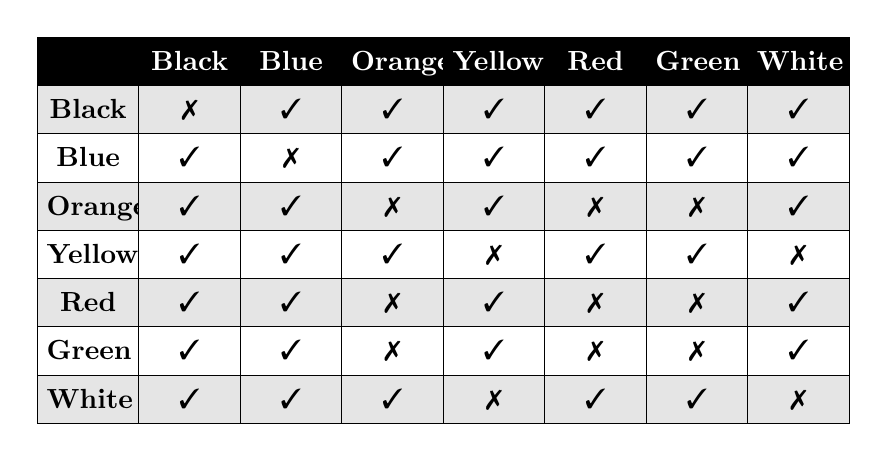
\begin{tikzpicture}
\matrix (first) [table,text width=3em]
{
& Black & Blue & Orange & Yellow & Red & Green & White\\
Black 	& \xmark & \cmark & \cmark & \cmark & \cmark & \cmark & \cmark \\
Blue   	& \cmark & \xmark & \cmark & \cmark & \cmark & \cmark & \cmark \\
Orange  & \cmark & \cmark & \xmark & \cmark & \xmark & \xmark & \cmark \\
Yellow  & \cmark & \cmark & \cmark & \xmark & \cmark & \cmark & \xmark \\
Red   	& \cmark & \cmark & \xmark & \cmark & \xmark & \xmark & \cmark \\
Green   & \cmark & \cmark & \xmark & \cmark & \xmark & \xmark & \cmark\\
White   & \cmark & \cmark & \cmark & \xmark & \cmark & \cmark & \xmark\\
};
\end{tikzpicture}
\captionof{figure}{Sample Look Up Table}
\label{Tick}

\section{SECTION-TITLE}
\label{SECTION-LABEL}

\section{SECTION-TITLE}
\label{SECTION-LABEL}

\subsection{SECTION-TITLE}
\label{SECTION-LABEL}

\subsection{SECTION-TITLE}
\label{SECTION-LABEL}
\cleardoublepage
\chapter{Evaluation}
\thispagestyle{plain}

\label{Evaluation}

To evaluate the approaches developed, we processed web pages using Kuhn's tool, SPRWeb and our tool and then compared the web pages on factors such as naturalness, differentiability, subjective naturalness and subjective differentiability.

\section{Improvements in SPRWeb}
\label{Improvements in SPRWeb}
We compared our tool with Kuhn’s[8] re-coloring tool.  Metrics of comparison were perceptual naturalness, perceptual differentiability, subjective naturalness and subjective differentiability as defined in definitions section in Chapter 2. 

\begin{table}[!htb]
\caption{Evaluation: Improvements in SPRWeb (numbers in scaled CIELAB euclidean distance)}
% title of Table
\centering
% used for centering table
\begin{tabular}{c c c c c c c c c}
% centered columns (4 columns)
\hline\hline
%inserts double horizontal lines
Web Page & N-k & N-t & D-k & D-t & SN-k & SN-t & SD-k & SD-t\\ [0.5ex]
% inserts table
%heading
\hline
% inserts single horizontal line
Complex 1 & 34 & 16 & 18 & 2.64 & 0.87 & 0.5 & 0.05 & 0.2 \\
% inserting body of the table
Complex 2 & 23 & 10 & 12 & 2.11 & 0.84 & 0.6 & 0.02 & 0.3\\
Complex 3 & 30 & 11 & 14 & 0.7 & 0.88 & 0.4 & 0.05 & 0.1\\
Complex 4 & 50 & 3 & 50 & 0.5 & 4 & 0.08 & 3.5 & 0.02\\
Complex 5 & 50 & 16 & 50 & 4.5 & 4 & 0.6 &1.3 & 0.2\\
Complex 6 & 33 & 8 & 20 & 0.3 & 1.23 & 1.04 & 0.14 & 0.3\\
Complex 7 & 47 & 16 & 17 & 2.15 & 0.87 & 1.01 & 0.018 & 0.4\\
Complex 8 & 50 & 27 & 20 & 4.25 & 1.73 & 1.5 & 1.37 & 0.4\\
Complex 9 & 40 & 21 & 23 & 4 & 0.99 & 1.1 & 0.1 & 0.5\\
Complex 10 & 50 & 21 & 50 & 2.6 & 3.07 & 1.1 & 4 & 0.3\\
Complex 11 & 18 & 6 & 15 & 1.6 & 0.78 & 0.4 & 0.05 & 0.2\\
Complex 12 & 44 & 17 & 17 & 3.8 & 1.29 & 0.6 & 0.02 & 0.2\\
Complex 13 & 27 & 12 & 23 & 1.7 & 0.8 & 0.7 & 0.15 & 0.3\\
Complex 14 & 14 & 4 & 10 & 0.5 & 0.3 & 0.1 & 0.104 & 0.1\\ [1ex]
% [1ex] adds vertical space
\hline
%inserts single line
\end{tabular}
\label{table:nonlin}
\begin{tabular}{@{}>{$}l<{$}l@{}}
    $k$ & Kuhn's Tool\\
    $t$ & Our tool developed by improvements in SPRWeb\\
    $N$ & Naturalness\\
    $D$ & Differentiability\\
    $SN$ & Subjective Naturalness\\
    $SD$ & Subjective Differentiability\\
  \end{tabular}
% is used to refer this table in the text
\end{table}

First we converted the output colors obtained from both kuhn's[8] and our tool to CIELAB notation. To assess naturalness-preservation, we compared the L*a*b* Euclidean distance between each original color and its respective Kuhn[8] and our replacement colors. Lower distances represent better naturalness-preservation, i.e., the replacement color is more perceptually-similar to the original color.To test perceptual differentiability, we calculated the Euclidean distance between each pair of colors in each original website and determined the absolute difference between this distance and the equivalent color pair in the Kuhn[8] and our versions. Lower values represent better differentiability restoration, i.e., the replacement colors are as differentiable (not more or less differentiable) as the original colors. Fig 4.1 gives a better view of comparison of the two tools in perceptual factors. 

\begin{figure}[!htb]
\centering
\includegraphics[width=\linewidth]{bar1.png}
\caption{Perceptual factors comparison}
\label{fig:sub2}
\end{figure}

For theoretical subjective response, we followed the same procedure as in the case of perceptual factors. The major difference being that instead of using $L^{*}$,$a^{*}$ and $b^{*}$ as three dimensions, we used temperature, activity and weight as three dimensions to represent colors (as defined in chapter 2). For each of the color in original CSS, kuhn's[8] solution and our solution, we calculated the temperature, activity and weight factors. Then these three values are taken as one coordinate and same process as followed in  perceptual factors was followed. Fig 4.2 compares kuhn's tool and our tool in subjectivity measures. 

\begin{figure}[!htb]
\centering
\includegraphics[width=\linewidth]{bar2.png}
\caption{Subjective factors comparison}
\label{fig:sub2}
\end{figure}

Based on this theoretical analysis, we show that our tool brings time complexity improvements in SPRWeb (derived theoretically), without a decline in its performance quantitatively.  


\section{Pair-wised approach}
\label{Pair-wised apporach}

To evaluate our approach mentioned in section 3.2, we did analysis with two types of web pages - simple web pages and complex web pages. 

\subsection{Simple web pages}
\label{Simple web pages}

We generated simple web pages(Fig 4.3), having 3 colors in its layout with no text or images. Eight color schemes were used to generate 8 different web pages with similar structure. To test the subjectivity response preservation of tools being compared, we chose colors which were situated at extremities of Ou's subjective response model[]. As defined in chapter 2, colors are represented in three subjective response dimensions - activity, temperature and weight. And 8 color schemes were designed with colors at the extremities of subjective response dimensions. 

\begin{figure}
\centering
\begin{subfigure}{.5\textwidth}
  \centering
  \includegraphics[width=.5\linewidth]{screenshotofsimple1.png}
  \caption{Simple 1}
  \label{fig:sub1}
\end{subfigure}%
\begin{subfigure}{.5\textwidth}
  \centering
  \includegraphics[width=.5\linewidth]{screenshotofsimple2.png}
  \caption{Simple 2}
  \label{fig:sub2}
\end{subfigure}
\caption{Simple web pages}
\label{fig:test}
\end{figure}


Our tool and SPRWeb were compared this time on same metrics that were followed in section 4.1 and using the same method. Table 4.2 shows the testing results for simple web pages. 


\begin{table}[!htb]
\caption{Evaluation: Our approach (numbers in scaled CIELAB euclidean distance)}
% title of Table
\centering
% used for centering table
\begin{tabular}{c c c c c c c c c c c}
% centered columns (4 columns)
\hline\hline
%inserts double horizontal lines
Web Page & C\# & P\# & N-S & N-t & D-S & D-t & SN-S & SN-t & SD-S & SD-t\\ [0.5ex]
% inserts table
%heading
\hline
Simple 1&3&2&44.89&52.02&5.78&0.11&0.06&0.29&2.84&3.07\\
Simple 2&3&2&19.23&20.37&4.35&0.04&1.02&0.63&1.74&1.82\\
Simple 3&3&2&78.11&71.24&7.66&0.09&1.08&0.76&2.03&2.54\\
Simple 4&3&2&21.03&30.27&14.19&0.006&1.87&1.92&0.95&1.25\\
Simple 5&3&2&74.7&59.76&0.33&0.15&1.1&2.05&3.38&3.26\\
Simple 6&3&2&20.41&28.16&0.11&0.009&1.43&1.66&1.8&1.94\\
Simple 7&3&2&63.46&78.98&0.003&0.13&2.31&2.52&2.57&2.73\\
Simple 8&3&2&24.67&38.17&8.35&0.04&2.44&2.95&1.29&1.37\\[1ex]
\hline
%inserts single line
\end{tabular}
\label{table:nonlin}
\begin{tabular}{@{}>{$}l<{$}l@{}}
    $S$ & SPRWeb\\
    $t$ & Our tool developed on parsing pairs of colors concept\\
    $N$ & Naturalness\\
    $D$ & Differentiability\\
    $SN$ & Subjective Naturalness\\
    $SD$ & Subjective Differentiability\\
  \end{tabular}
% is used to refer this table in the text
\end{table}

A comparison graph is given in Fig 4.4 (perceptual) and Fig 4.5(subjective).

\begin{figure}[!htb]
  \centering
  \includegraphics[width=\linewidth]{SimpleGP.png}
  \caption{Perceptual comparison}
  \label{fig:sub1}
\end{figure}

\begin{figure}[!htb]
  \centering
  \includegraphics[width=\linewidth]{simpleGS.png}
  \caption{Subjective comparison}
  \label{fig:sub2}
\end{figure}


We also randomly generated 10 simple web pages to compare our tool with SPRWeb. The data is given in Table 4.3.

\begin{table}[!htb]
\caption{Evaluation: Our approach (numbers in scaled CIELAB euclidean distance)}
% title of Table
\centering
% used for centering table
\begin{tabular}{c c c c c c c c c c c}
% centered columns (4 columns)
\hline\hline
%inserts double horizontal lines
Web Page & C\# & P\# & N-S & N-t & D-S & D-t & SN-S & SN-t & SD-S & SD-t\\ [0.5ex]
% inserts table
%heading
\hline
Simple 1&3&2&16.6&15.51&0.04&0.04&1.77&1.27&0.83&0.74\\
Simple 2&3&2&25.2&21.91&0.15&0.02&0.42&0.36&0.05&0.62\\
Simple 3&3&2&24.96&23.76&0.2&0.18&0.24&0.39&0.75&0.65\\
Simple 4&3&2&15.78&72.16&0.06&0.08&0.08&2.05&0.75&1.6\\
Simple 5&3&2&29.33&29.58&10.43&0.14&0.08&0.36&0.92&0.95\\
Simple 6&3&2&46.21&38.87&0.23&0.11&1.26&2.1&1.48&1.73\\
Simple 7&3&2&44.58&40.93&0.18&0.02&0.05&1.12&1.47&1.71\\
Simple 8&3&2&26.89&27.62&5.11&0.04&0.52&0.57&0.9&0.95\\
Simple 9&3&2&25.87&28.14&0.08&0.14&1.41&0.5&0.77&0.96\\
Simple 10&3&2&16.14&17.81&6.76&0.02&0.4&0.33&0.54&0.63\\[1ex]
\hline
%inserts single line
\end{tabular}
\label{table:nonlin}
\begin{tabular}{@{}>{$}l<{$}l@{}}
    $S$ & SPRWeb\\
    $t$ & Our tool developed on parsing pairs of colors concept\\
    $N$ & Naturalness\\
    $D$ & Differentiability\\
    $SN$ & Subjective Naturalness\\
    $SD$ & Subjective Differentiability\\
  \end{tabular}
% is used to refer this table in the text
\end{table}

A comparison plot is given in Fig 4.6 (perceptual) and Fig 4.7 (Subjective). 


\begin{figure}[!htb]
\centering
  \includegraphics[width=\linewidth]{simpleRP.png}
  \caption{Perceptual comparison}
  \label{fig:sub1}
\end{figure}

\begin{figure}[!htb]
  \centering
  \includegraphics[width=\linewidth]{simpleRS.png}
\caption{Subjective comparison}
\label{fig:test}
\end{figure}

Comparison of total cost can be seen in Fig 4.8 and Fig 4.9 for general and randomly generated web pages respectively. 


\begin{figure}[!htb]
\centering
  \includegraphics[width=\linewidth]{simpleGtotal.png}
  \caption{Total cost comparison for general pages}
  \label{fig:sub1}
\end{figure}

\begin{figure}[!htb]
  \centering
  \includegraphics[width=\linewidth]{simpleRtotal.png}
\caption{Total cost comparison for random pages}
\label{fig:test}
\end{figure}


It can be observed from the comparison that our tool performs better in maintaining perceptual differentiability in every case. The overall cost of our tool is less than that of SPRWeb in 12 out of 18 simple web pages. In 2 pages the cost is marginally greater than SPRWeb. It can also be observed that perceptual naturalness cost is significantly higher in our tool as compared to SPRWeb. This can be attributed to the step in the algorithm where we restrict our possible replacement set in order to preserve perceptual differentiability. 


\subsection{Complex web pages}
\label{Complex web pages}
In order to test our tool on real web pages, we selected 14 complex web pages. These web pages consisted of information style pages, forum-style pages and blog style pages. The evaluation data corresponding to these web pages is shown in Table 4.4. 
To test our tool further, we selected 18 more random complex pages and did analysis. Data corresponding to these 18 web pages is shown in Table 4.5. 


\begin{table}[!htb]
\caption{Evaluation: Our approach (numbers in scaled CIELAB euclidean distance)}
% title of Table
\centering
% used for centering table
\begin{tabular}{c c c c c c c c c c c}
% centered columns (4 columns)
\hline\hline
%inserts double horizontal lines
Web Page & C\# & P\# & N-S & N-t & D-S & D-t & SN-S & SN-t & SD-S & SD-t\\ [0.5ex]
% inserts table
%heading
\hline
Complex 1&12&12&29.05&29.05&8.22&0.05&1.08&2.11&1.21&1.26\\
Complex 2&12&9&10.28&11.18&5.08&0.11&1.29&0.94&0.73&0.72\\
Complex 3&4&3&9.15&7.77&0.24&0.1&0.41&0.65&0.28&0.32\\
Complex 4&6&4&7.88&8.66&5.12&0.02&0.31&0.11&0.3&0.39\\
Complex 5&6&4&10.78&10.49&0.079&0.015&0.35&0.71&0.28&0.34\\
Complex 6&7&4&10.19&9.73&2.63&0.05&1.38&2.16&0.92&0.92\\
Complex 7&22&22&21.57&23.99&67.46&0.01&7.35&8.89&1.39&1.48\\
Complex 8&5&4&34.81&46.3&22.7&0.02&1.1&2.32&1.85&2.5\\
Complex 9&7&5&32.5&34.83&28.22&0.08&2.25&0.705&1.57&1.61\\
Complex 10&6&5&13.09&17.29&17.25&0.05&1.68&0.54&0.71&0.649\\
Complex 11&15&15&25.12&27.79&9.88&0.61&0.87&1.15&3.28&4.52\\
Complex 12&13&9&24.45&30.98&15.38&0.24&0.8&1.1&0.9&0.4\\
Complex 13&9&7&13.56&21.33&1.62&0.002&0.77&1.1&1.21&0.62\\
Complex 14&13&10&16.76&17.6&41.62&0.09&0.78&0.82&0.82&0.06\\[1ex]
\hline
%inserts single line
\end{tabular}
\label{table:nonlin}
\begin{tabular}{@{}>{$}l<{$}l@{}}
    $S$ & SPRWeb\\
    $t$ & Our tool developed on parsing pairs of colors concept\\
    $N$ & Naturalness\\
    $D$ & Differentiability\\
    $SN$ & Subjective Naturalness\\
    $SD$ & Subjective Differentiability\\
  \end{tabular}
% is used to refer this table in the text
\end{table}


\begin{table}[!htb]
\caption{Evaluation: Our approach (numbers in scaled CIELAB euclidean distance)}
% title of Table
\centering
% used for centering table
\begin{tabular}{c c c c c c c c c c c}
% centered columns (4 columns)
\hline\hline
%inserts double horizontal lines
Web Page & C\# & P\# & N-S & N-t & D-S & D-t & SN-S & SN-t & SD-S & SD-t\\ [0.5ex]
% inserts table
%heading
\hline
Complex 1&5&3&9.92&9.65&2.49&0.14&1.09&1.02&0.72&0.77\\
Complex 2&10&9&17.51&18.68&40.7&0.08&2.9&1.62&0.87&1.06\\
Complex 3&12&11&29.15&33.21&133.05&0.44&6.33&2.02&1.41&1.46\\
Complex 4&16&17&15.79&15.95&36.8&0.06&4.6&4.02&0.89&0.9\\
Complex 5&8&7&30.22&46.14&69.48&0.35&7.41&6.34&1.62&1.91\\
Complex 6&11&9&1.92&2.19&0.48&0.14&5&5.54&0.48&0.5\\
Complex 7&15&8&11.57&12.44&1.89&0.03&0.91&0.69&1.17&1.18\\
Complex 8&11&12&3.2&3.26&0.56&0.05&0.73&0.11&0.2&0.36\\
Complex 9&8&10&10.39&21.05&20.98&0.24&0.39&6.25&0.83&1.03\\
Complex 10&15&11&24.99&33.76&61.53&0.01&4.6&4.94&1.41&1.78\\
Complex 11&8&9&8.76&9.38&2.34&0.15&0.49&0.68&0.61&0.65\\
Complex 12&16&17&12.73&12.69&14.98&0.4&6.35&5.35&0.87&0.94\\
Complex 13&13&15&3.57&3.7&0.71&0.005&1.01&6.65&0.1&0.24\\
Complex 14&16&12&0.14&0.41&0.089&0.45&0.029&0.86&0.003&0.11\\
Complex 15&10&9&20.62&24.46&1.21&0.03&1.6&1.81&0.99&1.31\\
Complex 16&16&10&22.21&32.2&26.85&0.1&1.23&2.84&1.09&1.42\\
Complex 17&3&3&1.61&12.57&0.32&0.042&0.06&2.51&0.09&0.49\\
Complex 18&16&11&5.33&5.99&0.24&0.4&1.35&2.16&0.16&0.33\\[1ex]
\hline
%inserts single line
\end{tabular}
\label{table:nonlin}
\begin{tabular}{@{}>{$}l<{$}l@{}}
    $S$ & SPRWeb\\
    $t$ & Our tool developed on parsing pairs of colors concept\\
    $N$ & Naturalness\\
    $D$ & Differentiability\\
    $SN$ & Subjective Naturalness\\
    $SD$ & Subjective Differentiability\\
  \end{tabular}
% is used to refer this table in the text
\end{table}

The comparison graphs are provided in Fig 4.10 (general perceptual), Fig 4.11 (general subjective), Fig 4.12 (random perceptual) and Fig 4.13 (random subjective).


\begin{figure}[!htb]
\centering
  \includegraphics[width=\linewidth]{complexGP.png}
  \caption{Perceptual comparison for general complex pages}
  \label{fig:sub1}
\end{figure}

\begin{figure}[!htb]
  \centering
  \includegraphics[width=\linewidth]{complexGS.png}
\caption{Subjective comparison for general complex pages}
\label{fig:test}
\end{figure}


\begin{figure}[!htb]
\centering
  \includegraphics[width=\linewidth]{complexRP.png}
  \caption{Perceptual comparison for random complex pages}
  \label{fig:sub1}
\end{figure}

\begin{figure}[!htb]
  \centering
  \includegraphics[width=\linewidth]{complexRS.png}
\caption{Subjective comparison for random complex pages}
\label{fig:test}
\end{figure}

Comparison of total cost for both general and random complex pages is provided in Fig 4.14 and Fig 4.15 respectively.

\begin{figure}[!htb]
\centering
  \includegraphics[width=\linewidth]{complexGtotal.png}
  \caption{Total cost comparison for general complex pages}
  \label{fig:sub1}
\end{figure}

\begin{figure}[!htb]
  \centering
  \includegraphics[width=\linewidth]{complexRtotal.png}
\caption{Total cost comparison for random complex pages}
\label{fig:test}
\end{figure}  

By analyzing the total cost comparison for complex web pages, we found that out of 32 pages, our tool performs better in 25 pages. While performs slightly poorer than SPRWeb in 4 pages. It can be observed that while the perceptual differentiability is better in every case for our tool and naturalness suffers. 

\section{Minimum Contrast}
\label{Minimum Contrast}



\subsection{SECTION-TITLE}
\label{SECTION-LABEL}

\subsection{SECTION-TITLE}
\label{SECTION-LABEL}

\cleardoublepage
\appendix
\include{sampleAppendix}
\cleardoublepage

\thispagestyle{plain}
\bibliographystyle{aaai}
\bibliography{sampleBibliography}

\end{document}
